\section{Information Visualisation}
Techniques for \emph{high-dimensional} data:
\begin{itemize}
\item Scatter plots, PCA
\item Parallel coordinates
\item Link+Brush
\item Pixel-oriented techniques
\item Icon-based techniques
\end{itemize}

Techniques for \emph{hierarchical} data and \emph{networks}
\begin{itemize}
\item Trees: Treemaps
\item Graph clustering
\item Distortion, Focus and Context
\end{itemize}

"Dimension" often refers to \emph{data channels} (attributes) and not to true \emph{spatial dimension} (coordinates).

Roles of data and coordinates can be swapped: In the \emph{data domain} the data becomes coordinates and vice versa.

\subsection{Scatter Plots}
Scatter plots or multi-dimensional histograms are projections of the attribute space to a 2D (or sometimes 3D) subspace.

Point density in scatter points is difficult to perceive. Colour coding of the density improves this somewhat especially in the high-density regions.

\emph{Continuous scatter plots} (Bachthaler) work also for low densities if the data has a spatial domain!

Idea: Modify the \emph{projected tetrahedra} algorithm. Instead of view projection transform to the data domain. 

Density at the thick vertex: ${1\over 3}$ Volume/Area$_\text{data domain}$.
\begin{figure}[H]
\centering
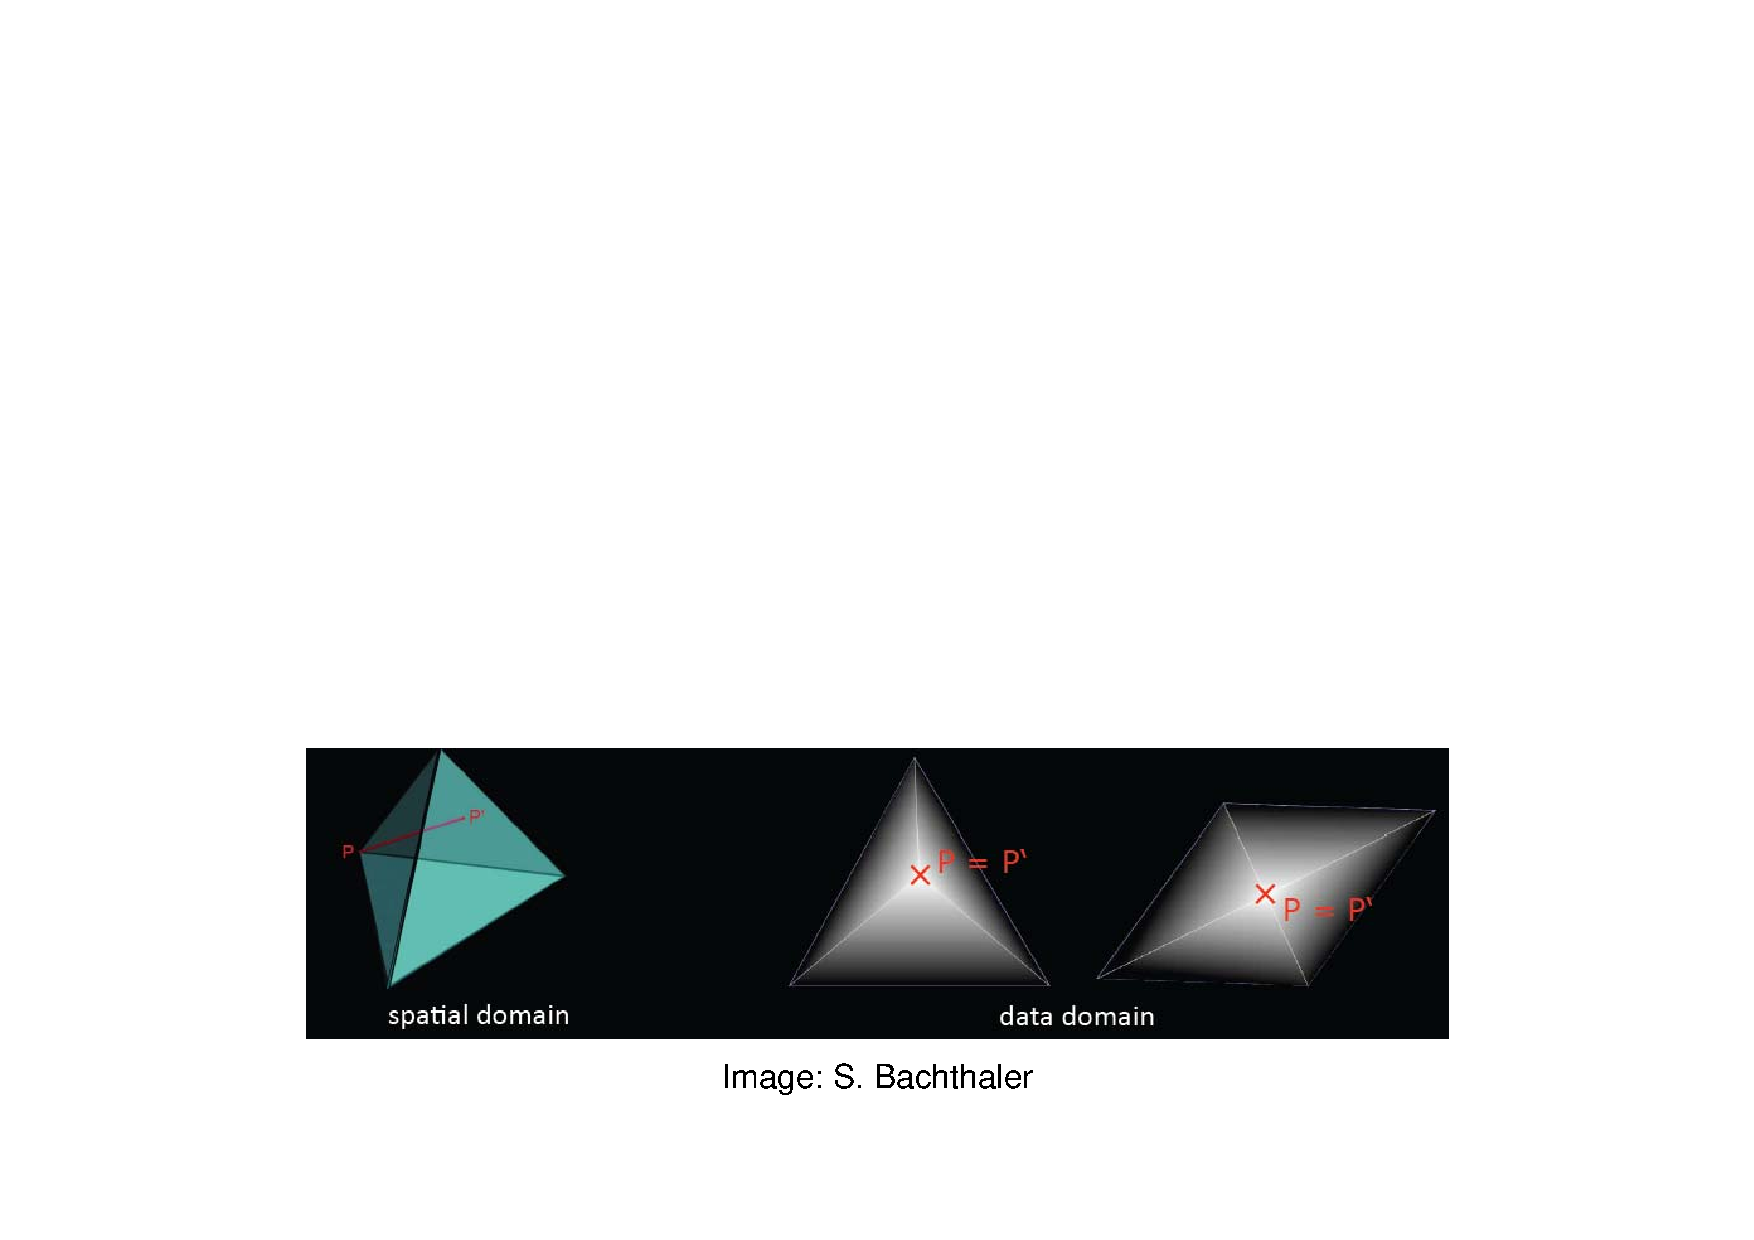
\includegraphics[width=0.8\textwidth]{img/12_continuous_scatter_plots}
\end{figure}

For $n>3$ a single scatter plot cannot be used. $n$-dimensional data leads to a $n\times n$ \emph{matrix} of 2D scatter plots.

For small $n$ the matrix can directly serve as a visualisation:
\begin{figure}[H]
\centering
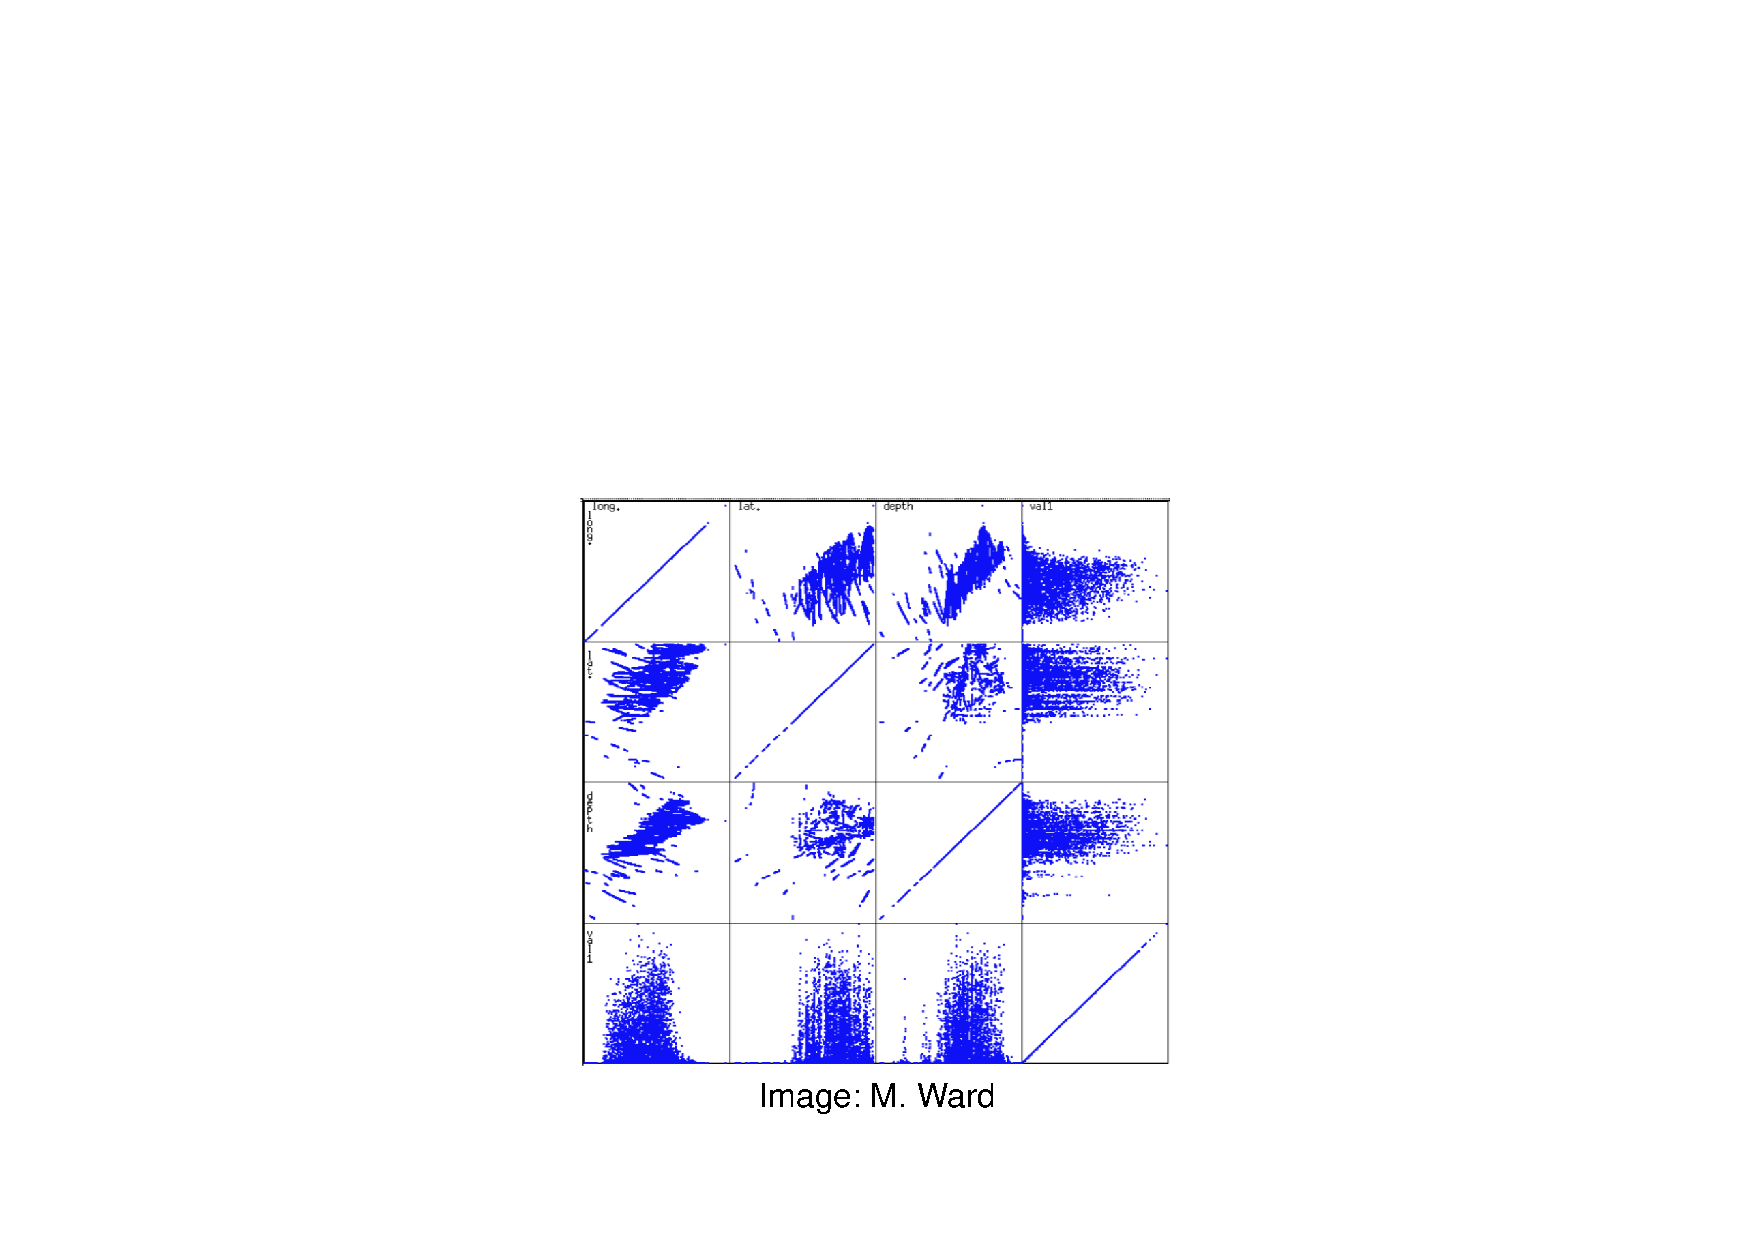
\includegraphics[width=0.5\textwidth]{img/12_scatter_plot_matrix}
\end{figure}

\subsection{Dimension Reduction}
See CIL.

\subsection{Parallel Coordinates}
Visualisation method of \emph{parallel coordinates} (Inselberg 1985):
\begin{itemize}
\item $n$ parallel and equidistant axes (one per attribute)
\item Axes scaled to $[\min,\max]$ range of corresponding attribute. 
\item Every data item is represented by a polyline which intersects each of the axes at the point corresponding to its attribute.
\end{itemize}
\begin{figure}[H]
\centering
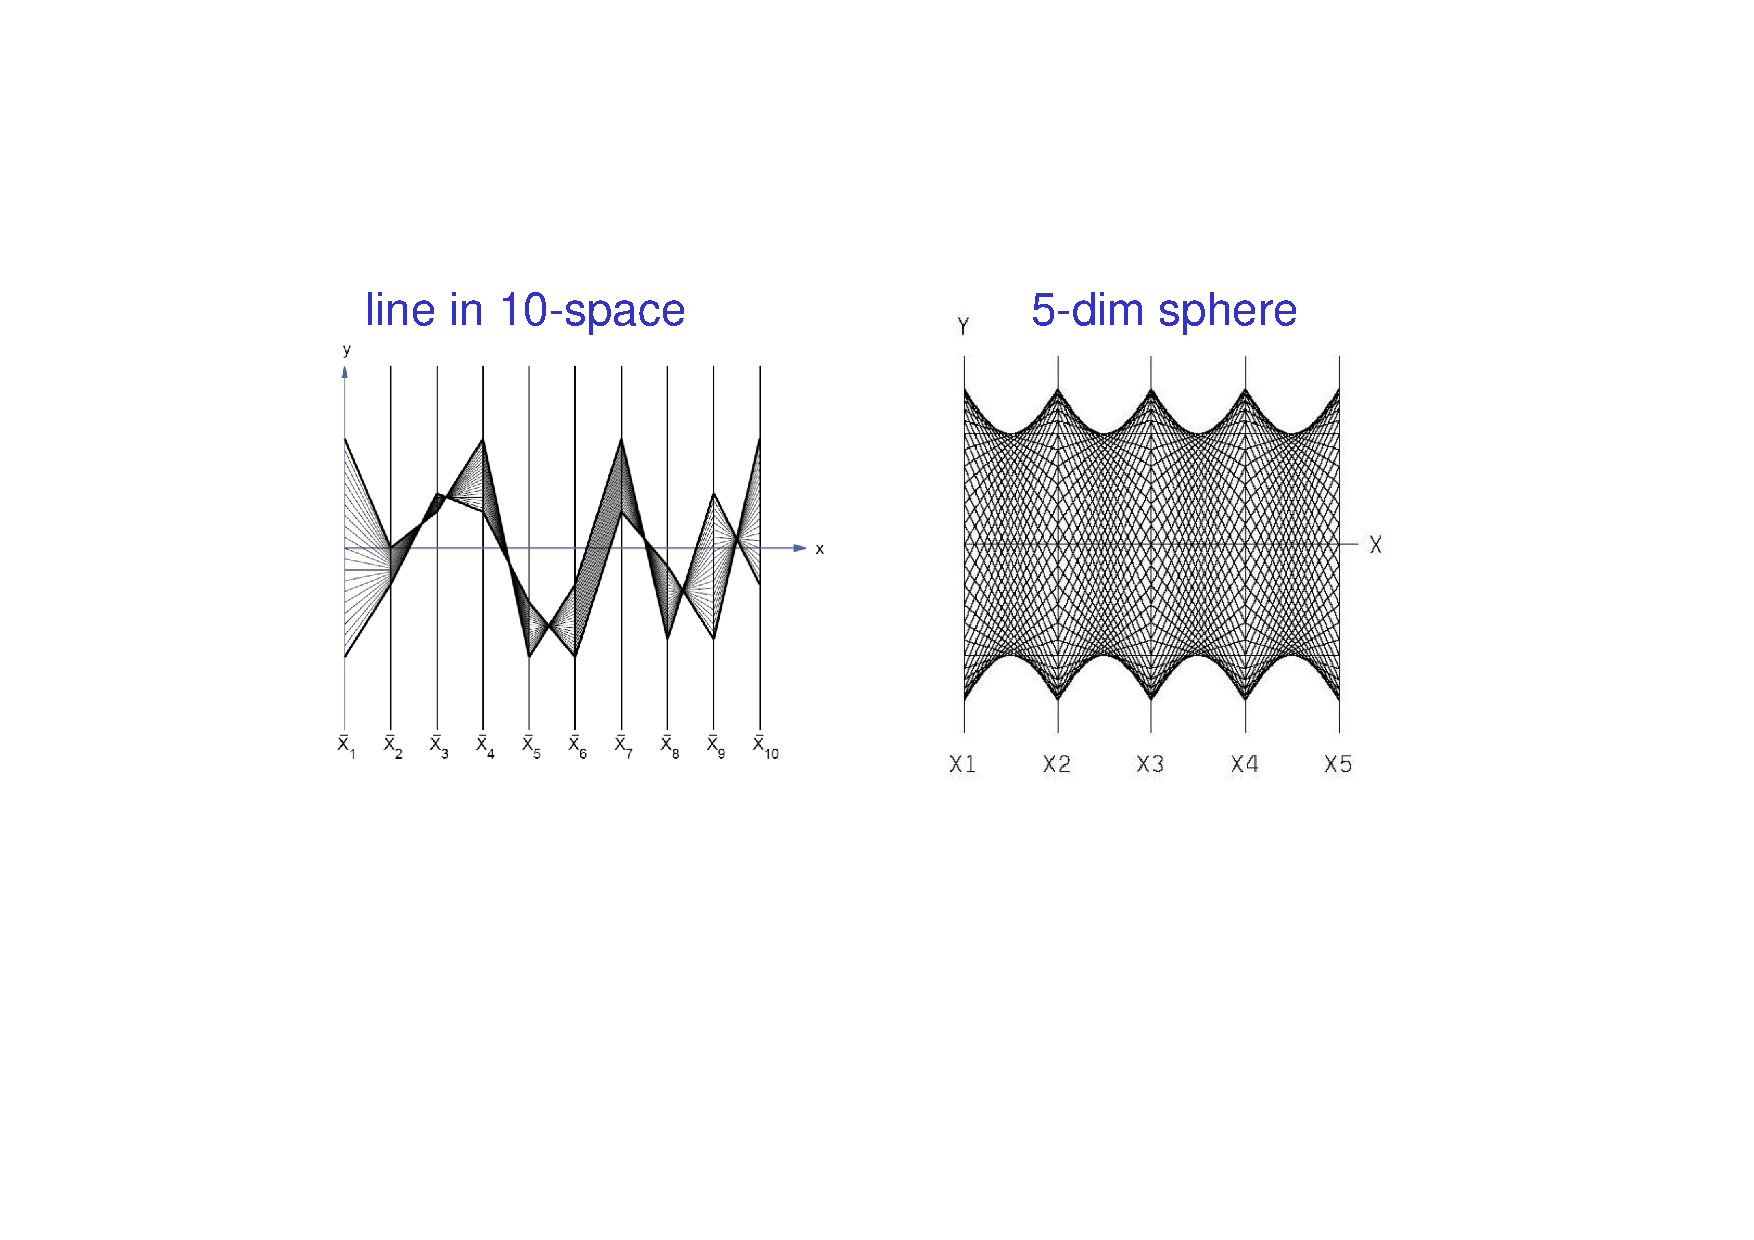
\includegraphics[width=0.6\textwidth]{img/12_parallel_coordinates}
\end{figure}

Linear or spherical arrangement can be "seen" (Inselberg). Algorithm for testing if a point is in the convex hull of a set of points: Check if the polyline is within the two envelopes of the set of polylines.

\subsection{Pixel-Oriented Techniques}
\subsubsection{Space-Filling Curves}
Represent each record by a single pixel. Map one attribute to a colour, map sorting key to space-filling curve.
\begin{itemize}
    \item Peano-Hilbert
    \item Z-Curve (Morton)
\end{itemize}
\subsubsection{Spiral Technique}
The spiral technique (Keim) for query dependent visualisation:
\begin{itemize}
\item Sort records (near a query point) by distance to query.
\item Map sorted list to spiral.
\end{itemize}

\subsubsection{Axes Technique}
For query dependent visualisation (Keim): 
\begin{itemize}
\item For two selected attributes separate space into lower/higher attribute values. 
\item Draw spirals per quarant.
\end{itemize}
\subsection{Icon-Based Techniques}
\subsubsection{Chernoff Faces}
\begin{itemize}
\item Two attributes are mapped to the display axes
\item Remaining attributes are mapped to shape and size of hair, eyebrows, eyes, nose, mouth, etc...
\end{itemize}

Idea: Use the human ability to recognise and memorise faces.
\begin{figure}[H]
\centering
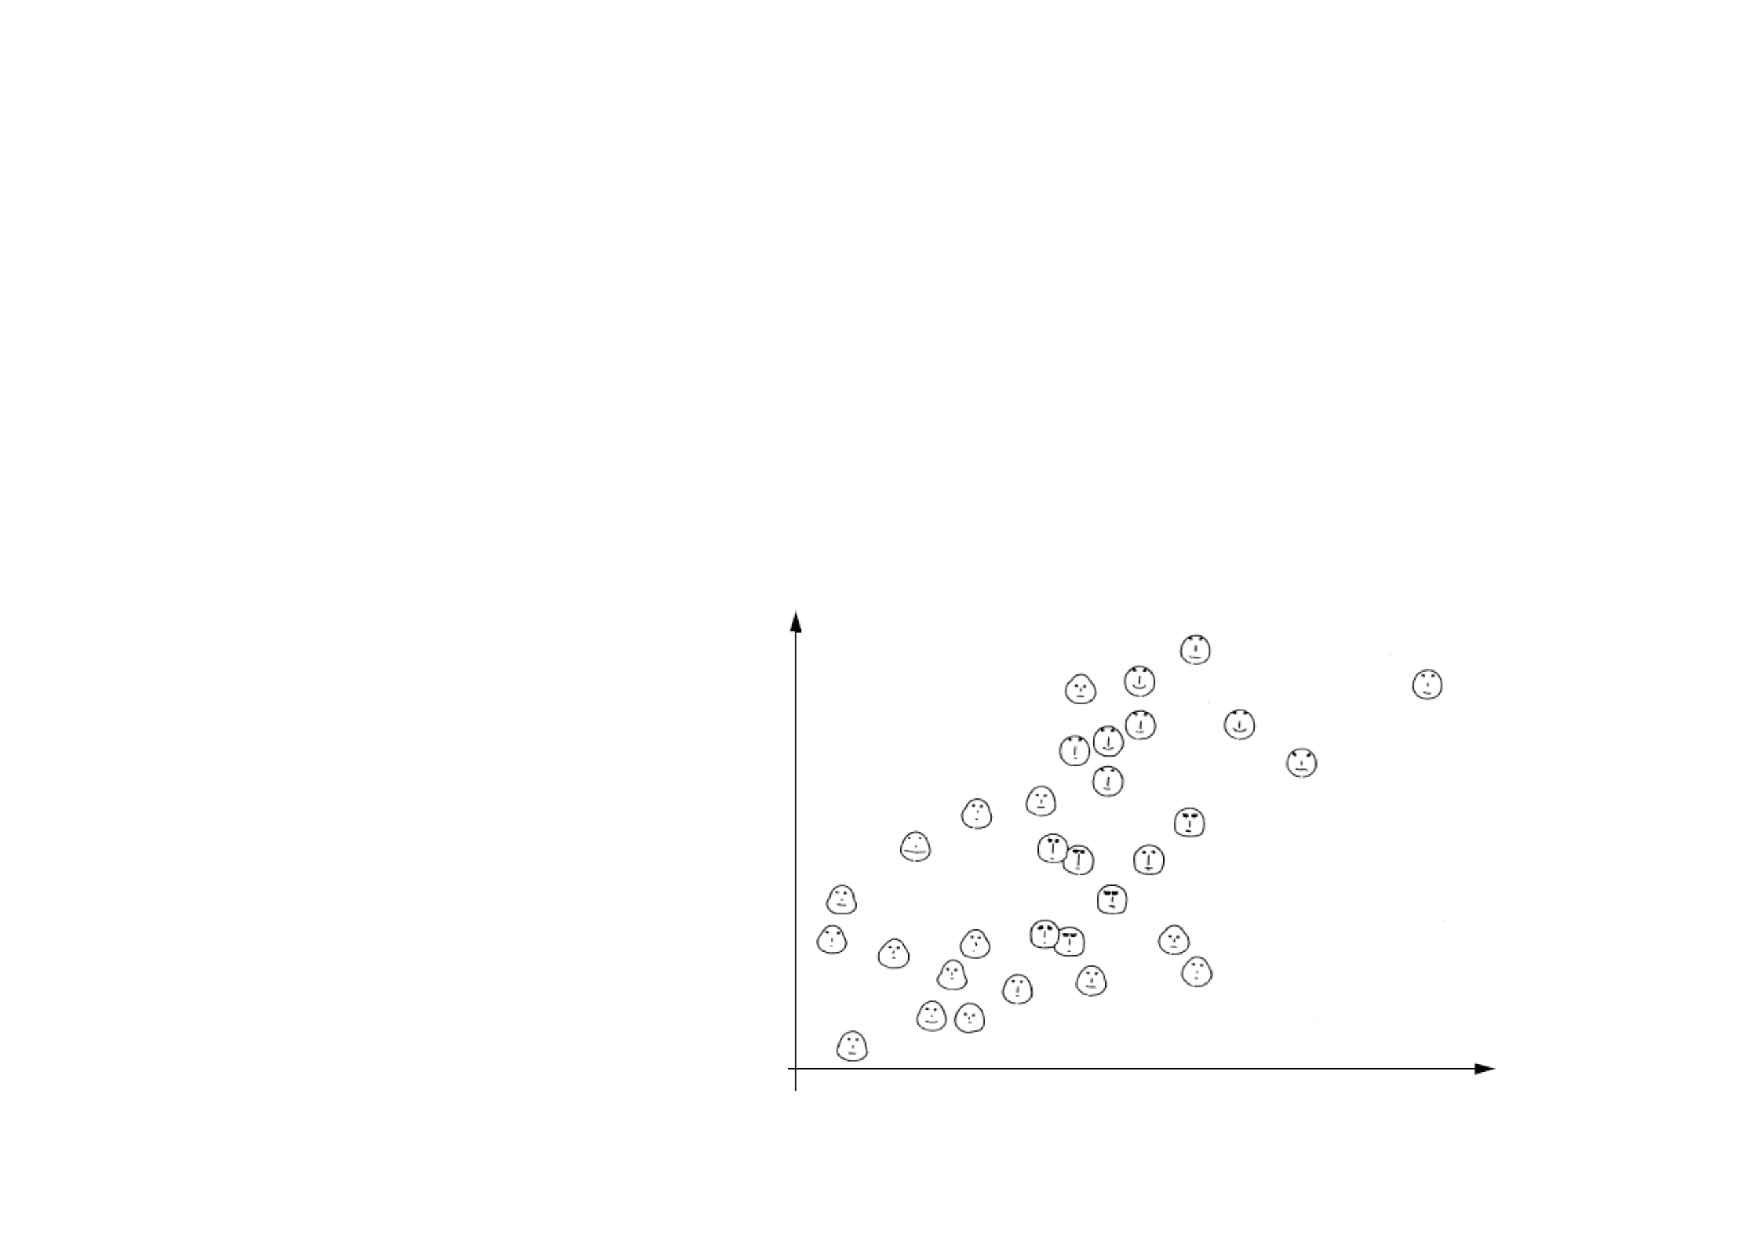
\includegraphics[width=0.7\textwidth]{img/12_chernoff_faces}
\end{figure}

\subsubsection{Stick Figures}
(Grinstein)
\begin{itemize}
\item Two attributes are mapped to the display axes.
\item The remaining attributes are mapped to lengths of limbs or angles between them.
\end{itemize}

Idea: Texture pattern in visualisation shows certain characteristics.

Example: Census data (age, income, sex, education, etc...)
\begin{figure}[H]
\centering
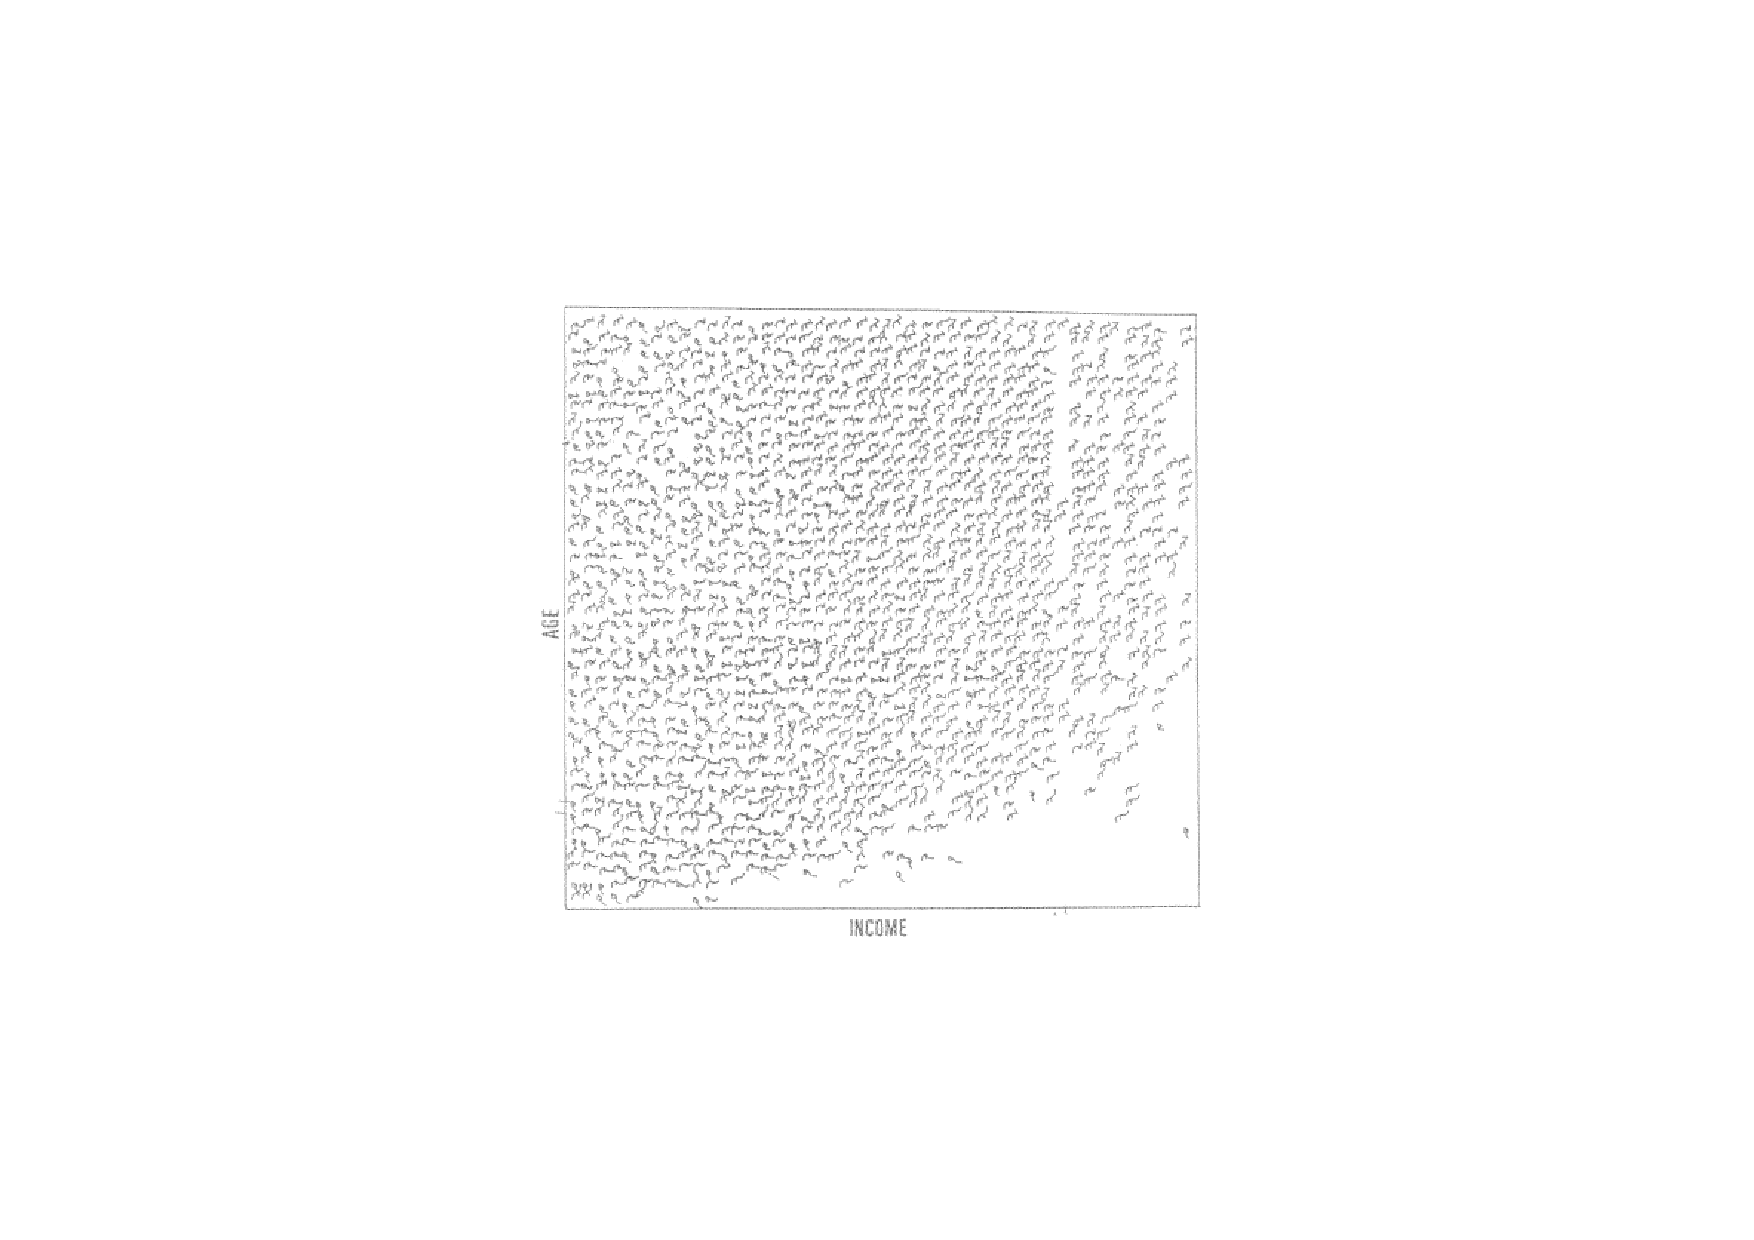
\includegraphics[width=0.7\textwidth]{img/12_stick_figures}
\end{figure}
It can be observed that the structure is more homogenous for higher incomes than for lower ones.

\subsection{Hierarchical and Network Data}
Mathematical description of hierarchies and networks: Graphs.

Some important special types of graphs:
\begin{itemize}
\item Undirected graphs
\item Directed graphs
\item Directed acyclic graphs (DAGs)
\item Rooted trees
\item Unrooted trees (i.e. every node can be chosen as the root)
\item Forests, etc..
\end{itemize}

\subsubsection{Cone Trees}
Cone trees (Robertson) are 3D embeddings of trees.
\begin{itemize}
\item Children are arranged on circular cones
\item Navigation by interactive roation at all hierarchy levels.
\end{itemize}

Useful for trees with high branching (no binary trees!).
\begin{figure}[H]
\centering
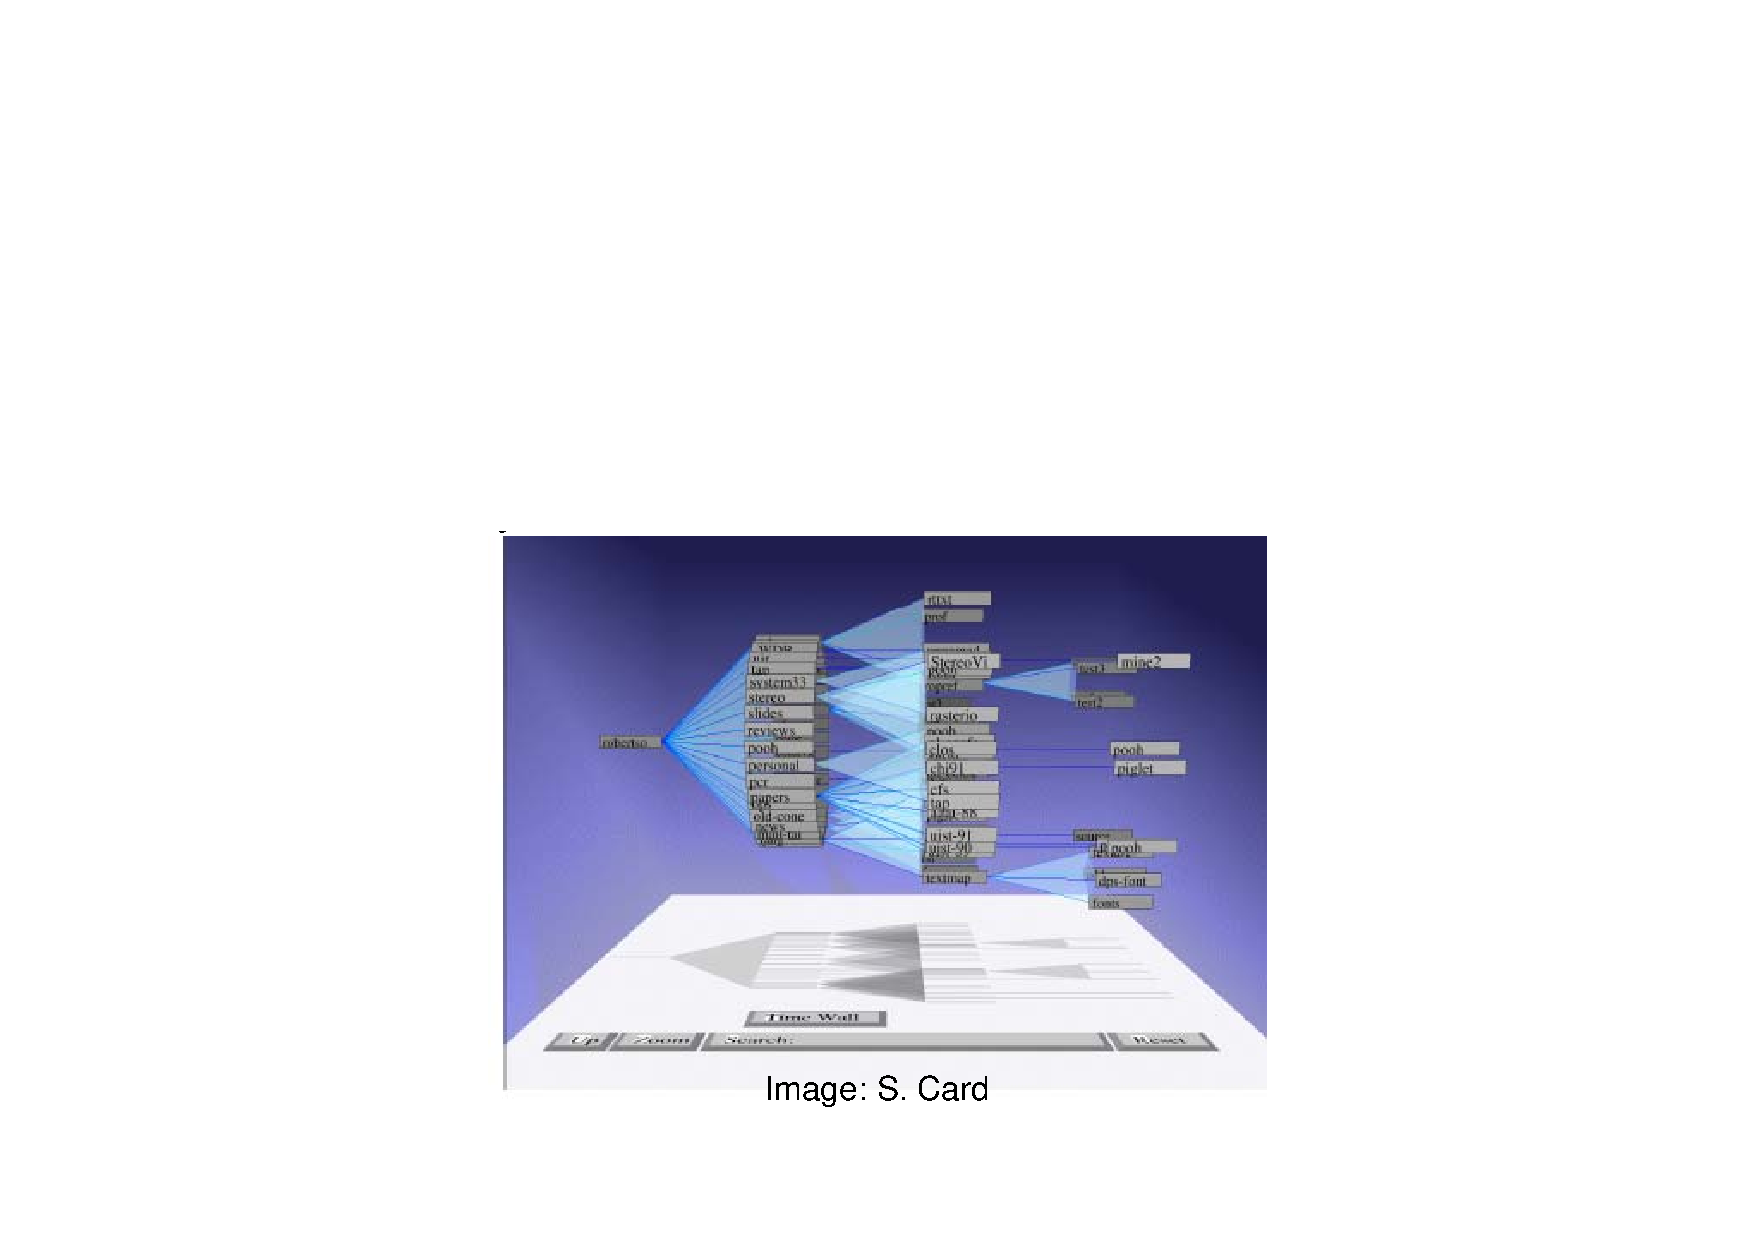
\includegraphics[width=0.7\textwidth]{img/12_cone_tree}
\end{figure}

\subsubsection{Tree Maps}
Trees with weight attribute at nodes can be visualised using \emph{tree maps} (Johnson and Shneiderman).

Tree maps are special Venn diagrams where
\begin{itemize}
\item Subtrees are represented by rectangles
\item Rectangle area is proportional to total weight of the subtree
\item Split direction is vertical/horizontal for odd/even hierarchy level
\item Nodes can have colours, labels, tool-tip info, etc...
\end{itemize}

Problem of tree maps:
 In large trees, hierarchical levels can be hard to see:
\begin{figure}[H]
\centering
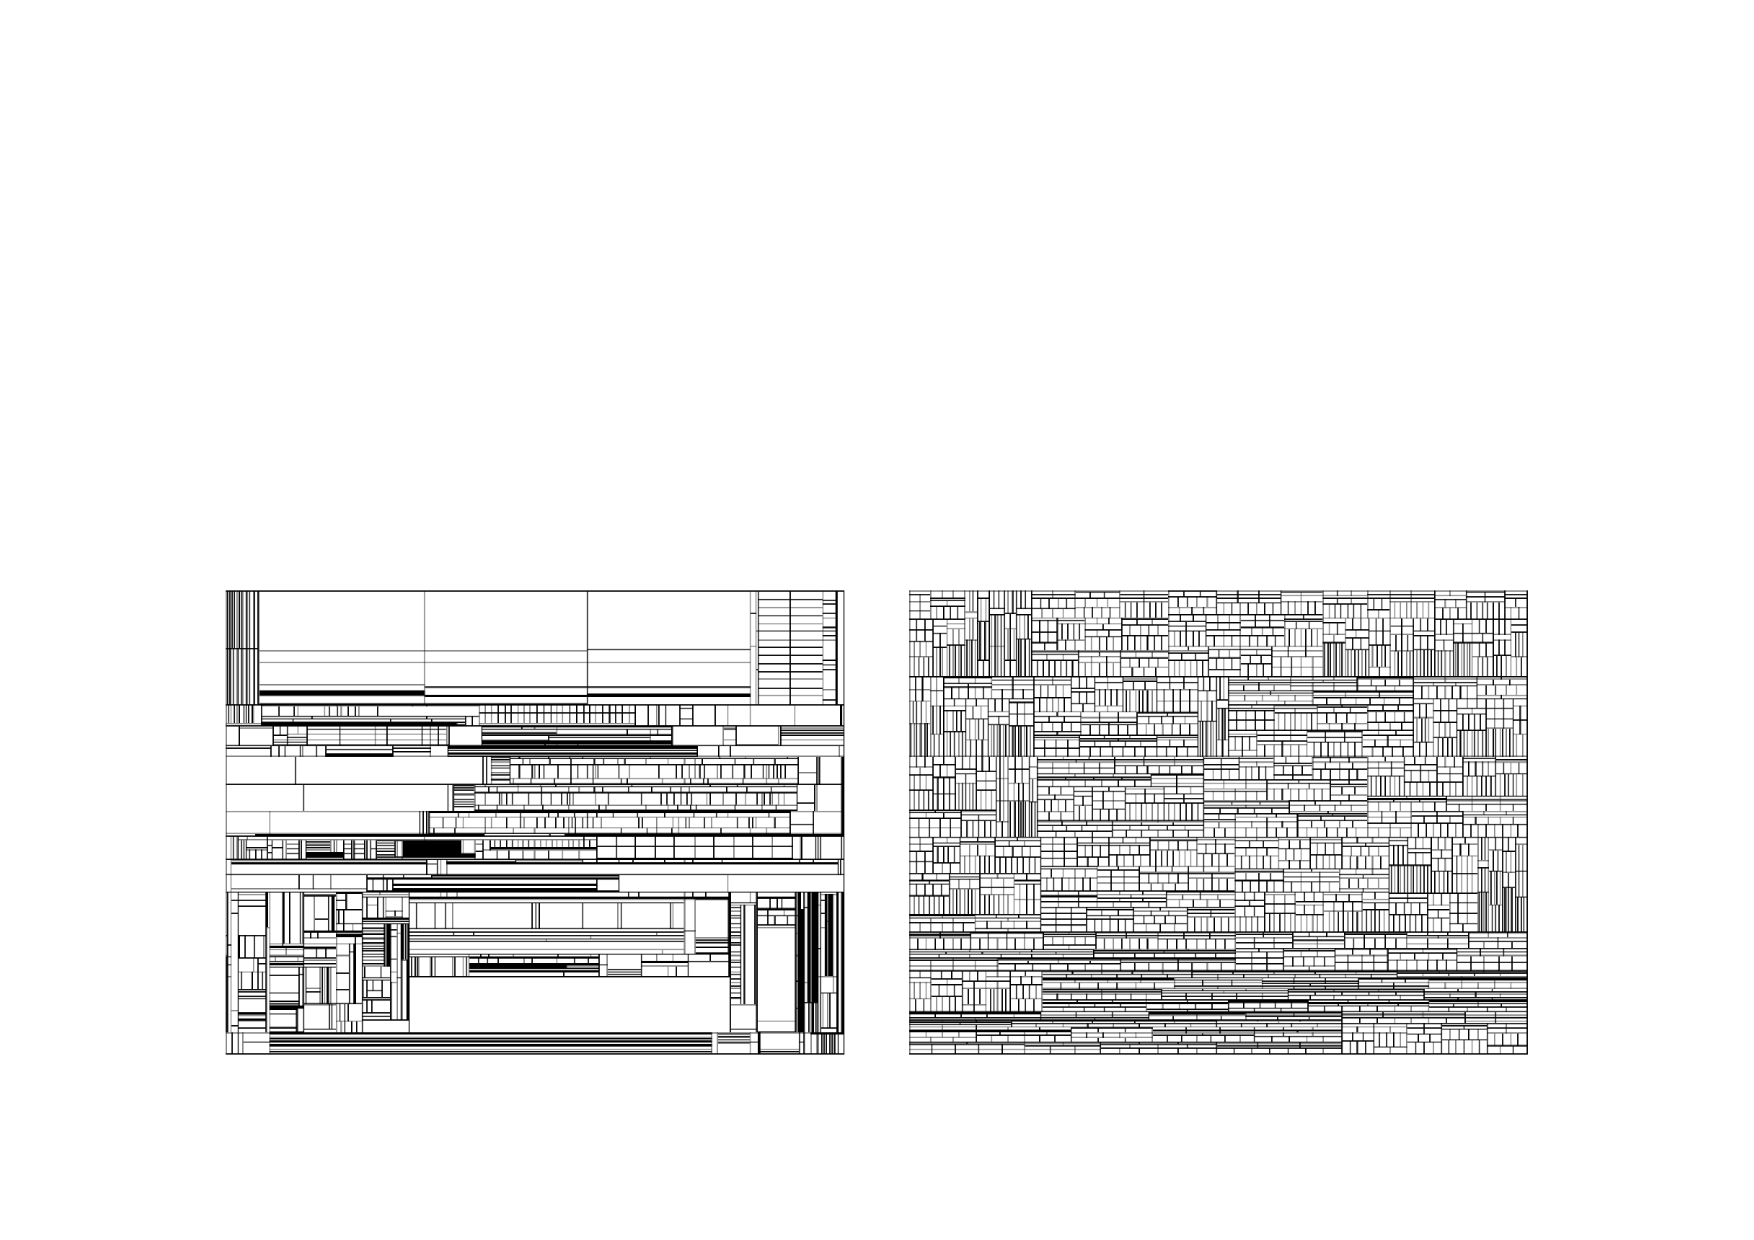
\includegraphics[width=0.7\textwidth]{img/12_tree_map_fs}
\end{figure}

Solution: \emph{Cushion tree maps} (van Wijk, van de Wetering 99).

Idea: Give rectangles a height profile with height depending on the hierarchy level.

Example (1D): Height profile for a binary tree.
\begin{figure}[H]
\centering
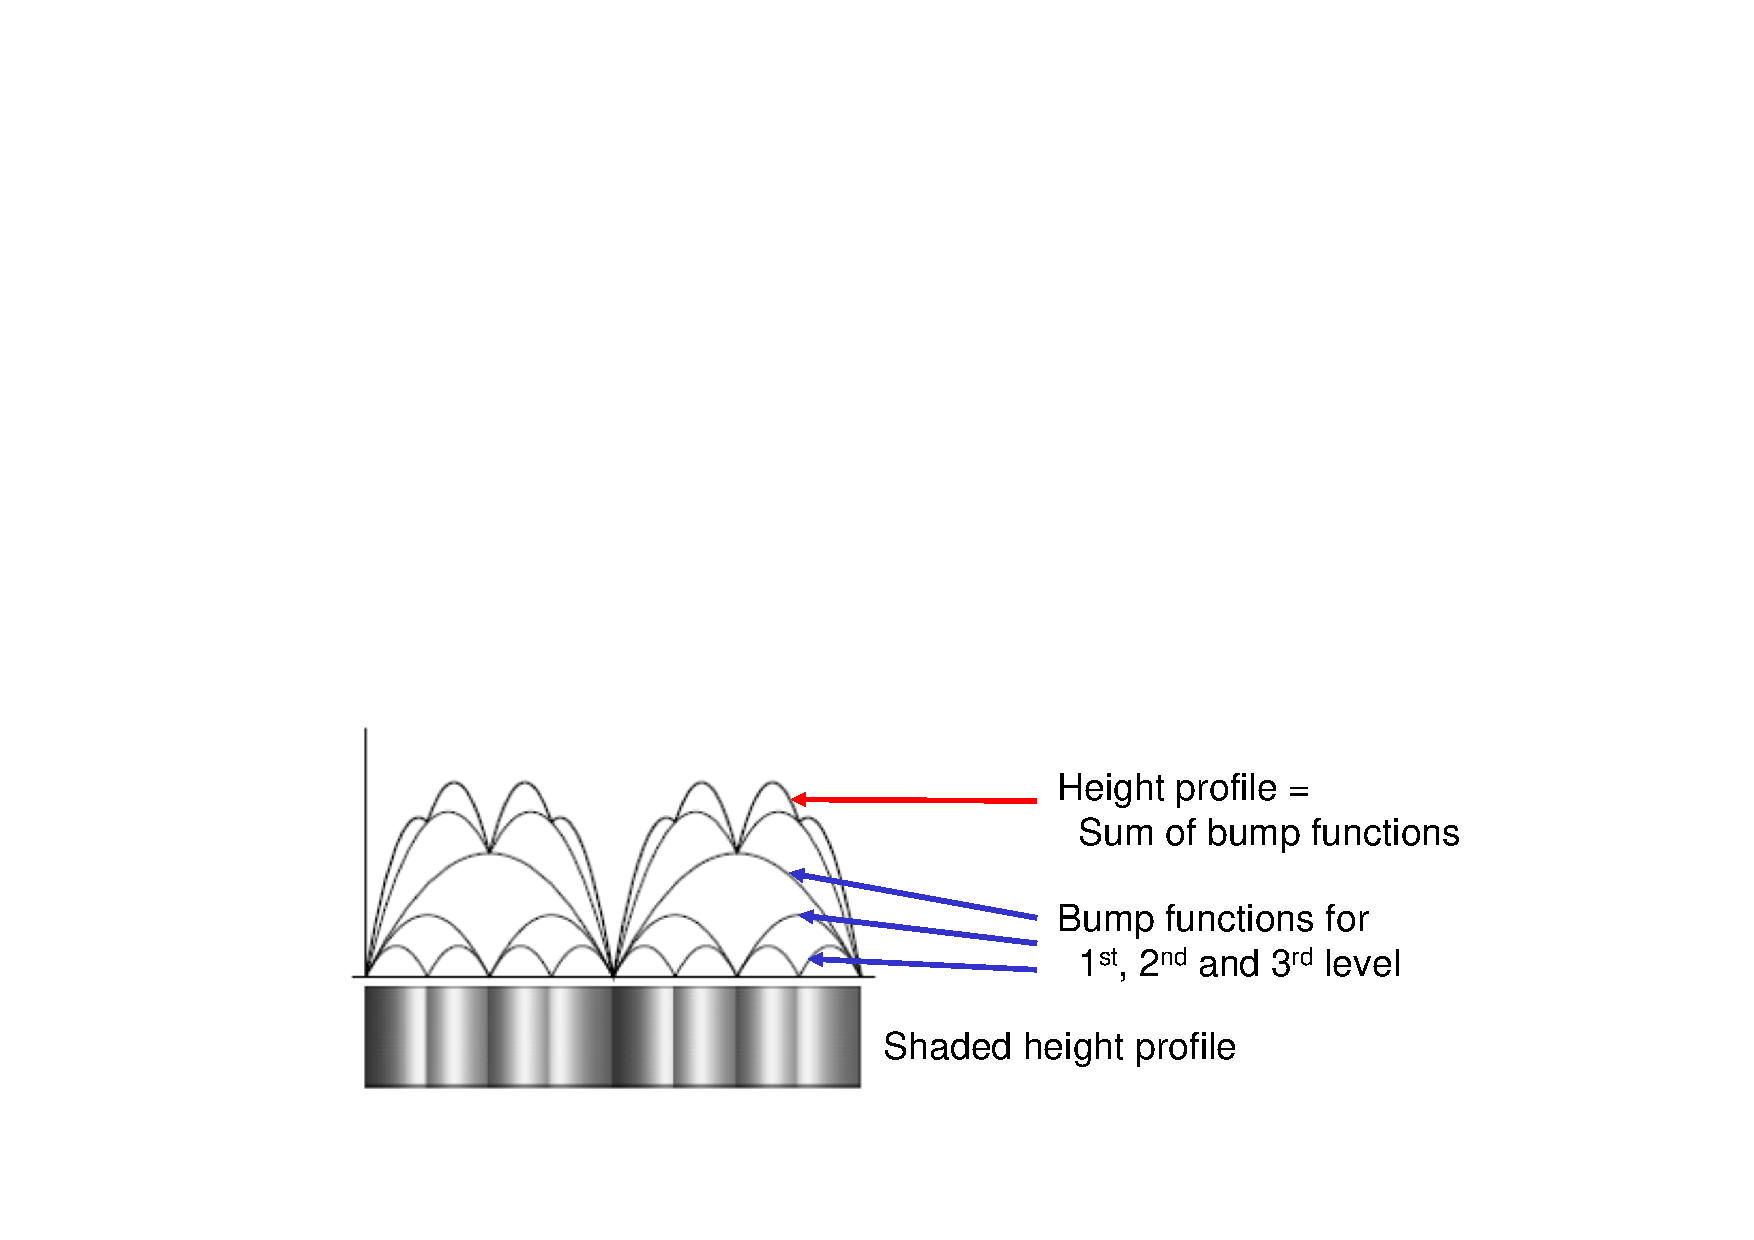
\includegraphics[width=0.7\textwidth]{img/12_cushion_tree_maps}
\end{figure}

$2^{nd}$ problem of tree maps: Bad aspect ratios. 

Solution: \emph{Squarified tree maps} (Bruls et al.).

Idea: Allow both vertical and horizontal splits within the same level of the tree.

Algorithm:
\begin{itemize}
\item Sort children by descending weight.
\item While list of children not empty:
\begin{itemize}
    \item Insert the first child, splitting the larger edge
    \item Repeat:
        \begin{itemize}
            \item "Squeeze" the next child into the same "row" (along the shorter edge)
            \item If aspect ratio is worse than that of the previous step, undo the step and break the inner loop.
        \end{itemize}
\end{itemize}
\end{itemize}

\begin{figure}[H]
\centering
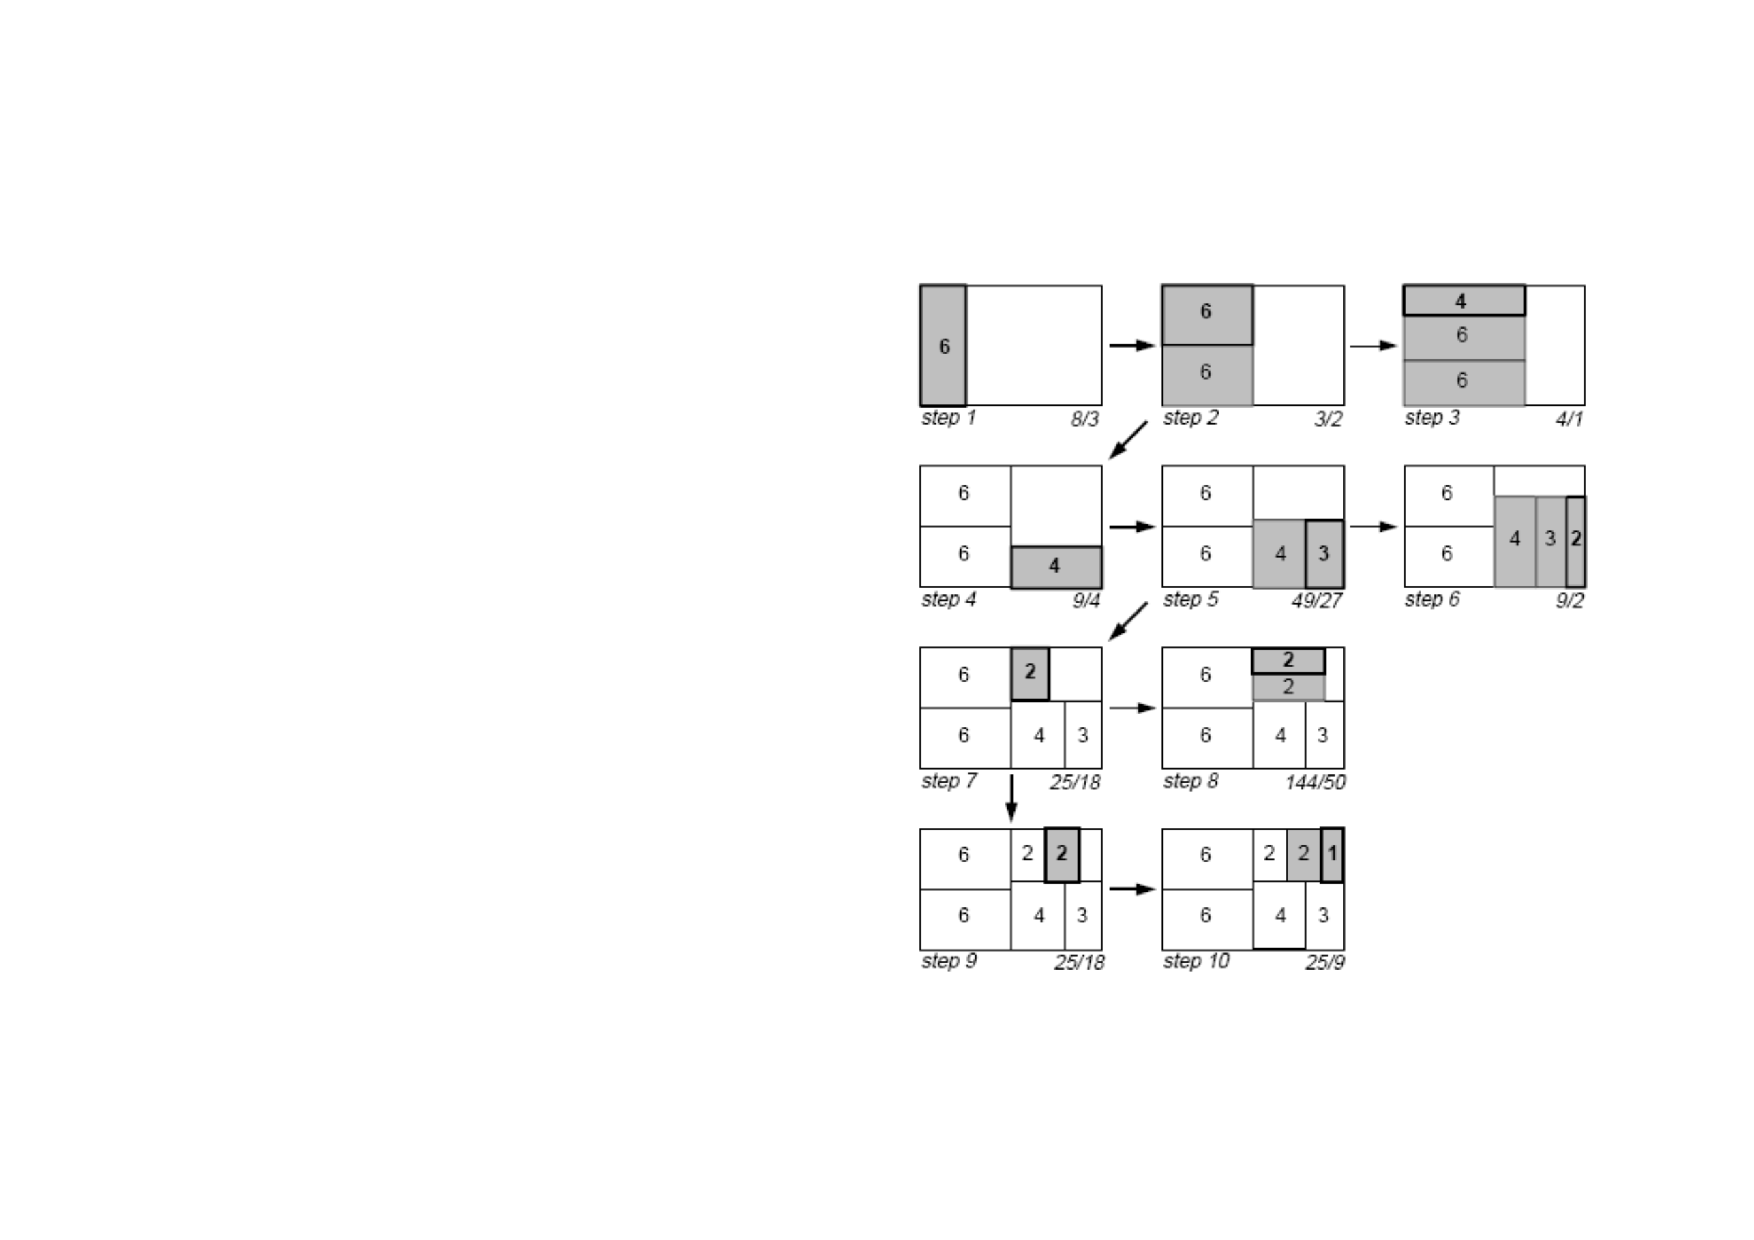
\includegraphics[width=0.7\textwidth]{img/12_squarified_tree_map}
\end{figure}

\subsection{Vornoi Tree Maps}
$S=\{s_1,\ldots,s_n\}$ is a set of "sites" (points) in $\R^2$. The cell generated by $s_i$ is:
\begin{align*}
    c_i = \left\{
        p\in \R^2: \norm{s_i-p} < \norm{s_j-p}\ (j\neq i)
    \right\}
\end{align*}

Example: Unbounded and bounded Voronoi tessellation:
\begin{figure}[H]
\centering
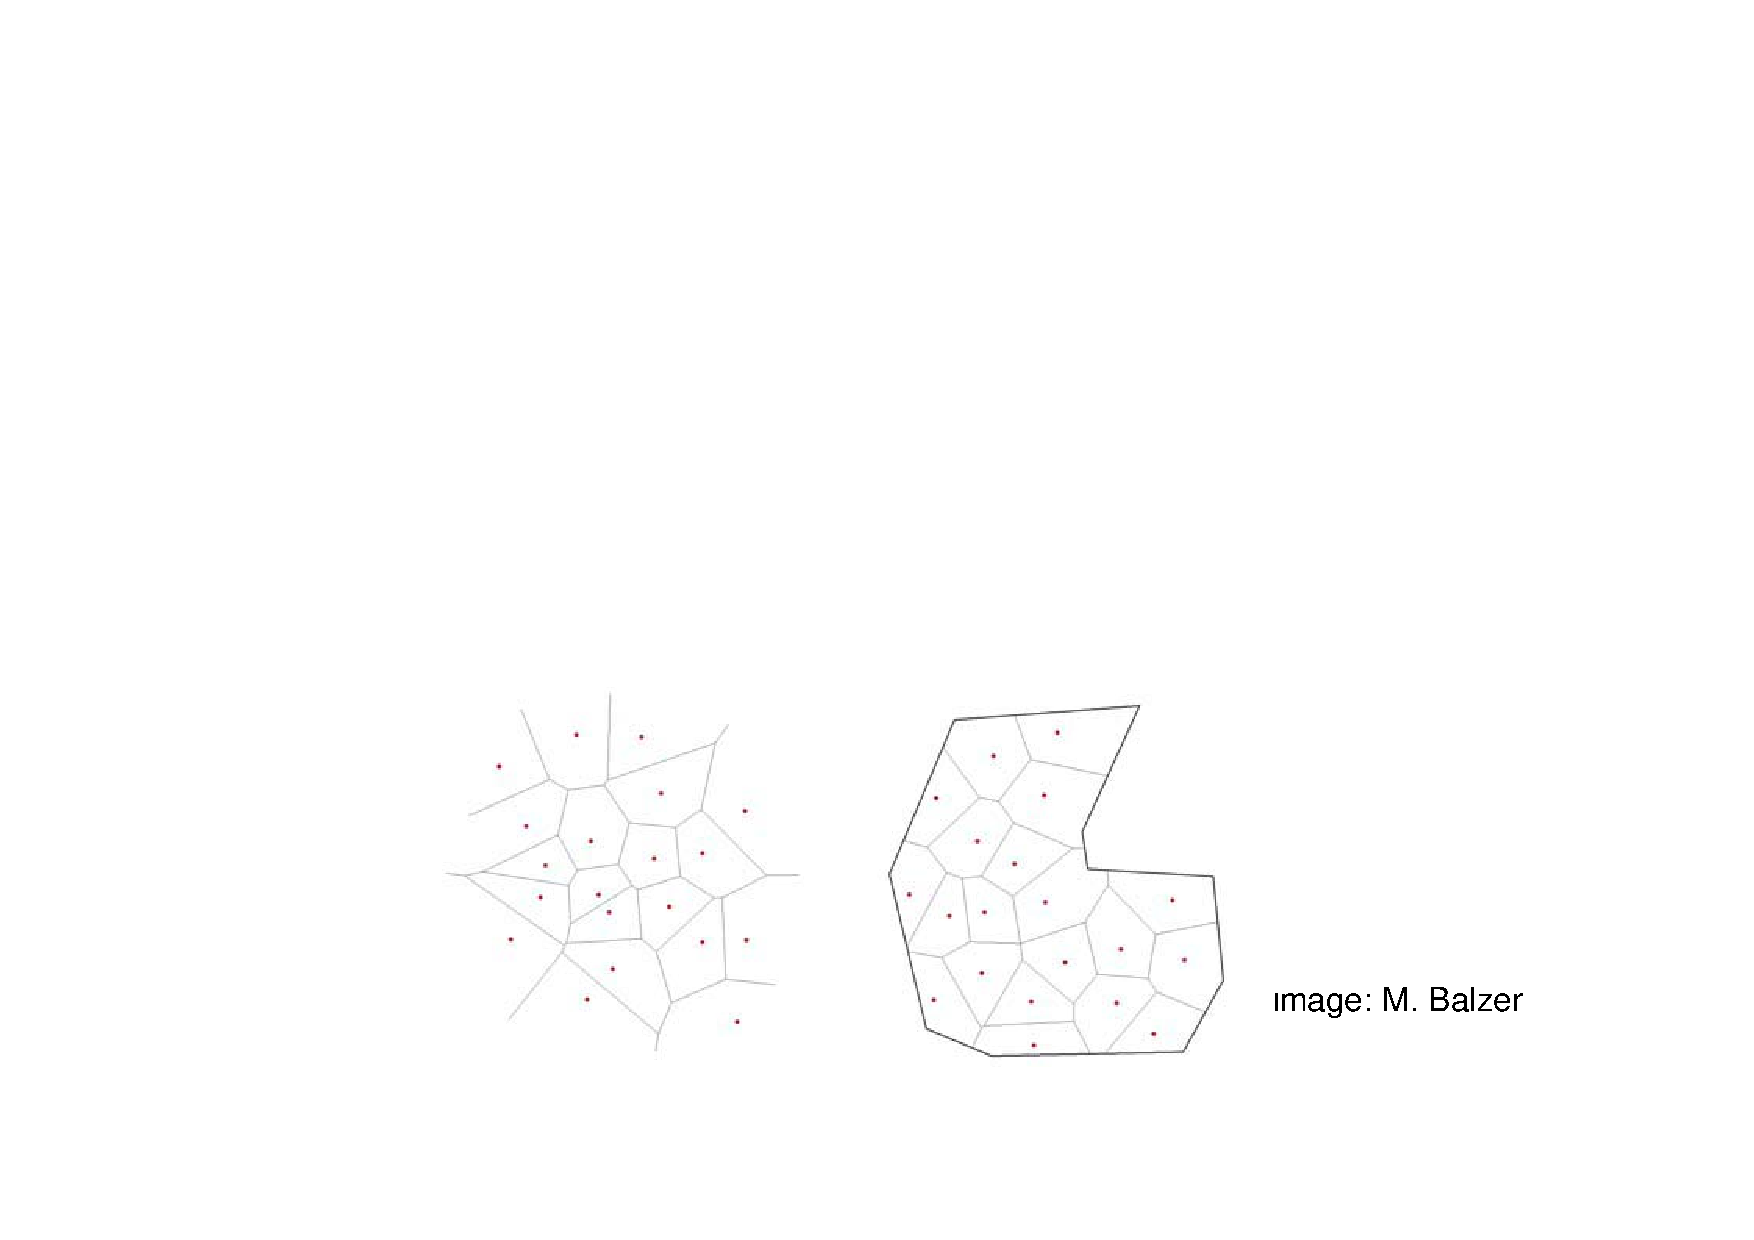
\includegraphics[width=0.7\textwidth]{img/12_voronoi_tessellation}
\end{figure}

\subsubsection{Additively Weighted (AW) Voronoi Tessellation}
Each site $s_i$ has a \emph{weight} $w_i$. The cell generated by $\langle s_i, w_i\rangle$ is:
\begin{align*}
    c_i = \left\{
        p\in \R^2: \norm{s_i-p}-w_i < \norm{s_j-p}-w_j\ (j\neq i)
    \right\}
\end{align*}

AW Voronoi tessellation is a generalised  Voronoi tessellation with circles as generators.

The edges are now hyperbola.

\subsubsection{Power Weighted (PW) Voronoi Tessellation}

The cell generated by $\langle s_i, w_i\rangle$ is:
\begin{align*}
    c_i = \left\{
        p\in \R^2: \norm{s_i-p}^2-w_i < \norm{s_j-p}^2-w_j\ (j\neq i)
    \right\}
\end{align*}

Weight now corresponds to squared radii of circles. The edges are now straight lines.



\subsubsection{Voronoi Tree Map}
\begin{itemize}
\item Start with initial cell representing the full tree.
\item Recursively subdivide the cell into AW or PW cells.
\item Use weights for controlling the area of cells.
\end{itemize}

Problem: The area of the cells differs from the circle area. Controlling the cell area is difficult.

Solution: Use a \emph{centroidal Voronoi tesselation} (CVT), where sites are at the centroids of cells. 
This results in "rounder" cells. 

Subdivision of a cell now requires an \emph{iteration}:
\begin{itemize}
\item Set initial weights according to tree attribute data.
\item Place sites "randomly within a cells (Additional complication: empty cells must be avoided).
\item Repeat:
    \begin{itemize}
        \item Compute AW or PW Voronoi tesselation
        \item Compute cell areas
        \item Compute errors (=deviation from intended areas)
        \item Adjust weights
        \item Replace sites by cell centroids
    \end{itemize}
    
    until errors $<$ tolerance.
\end{itemize}

\begin{figure}[H]
\centering
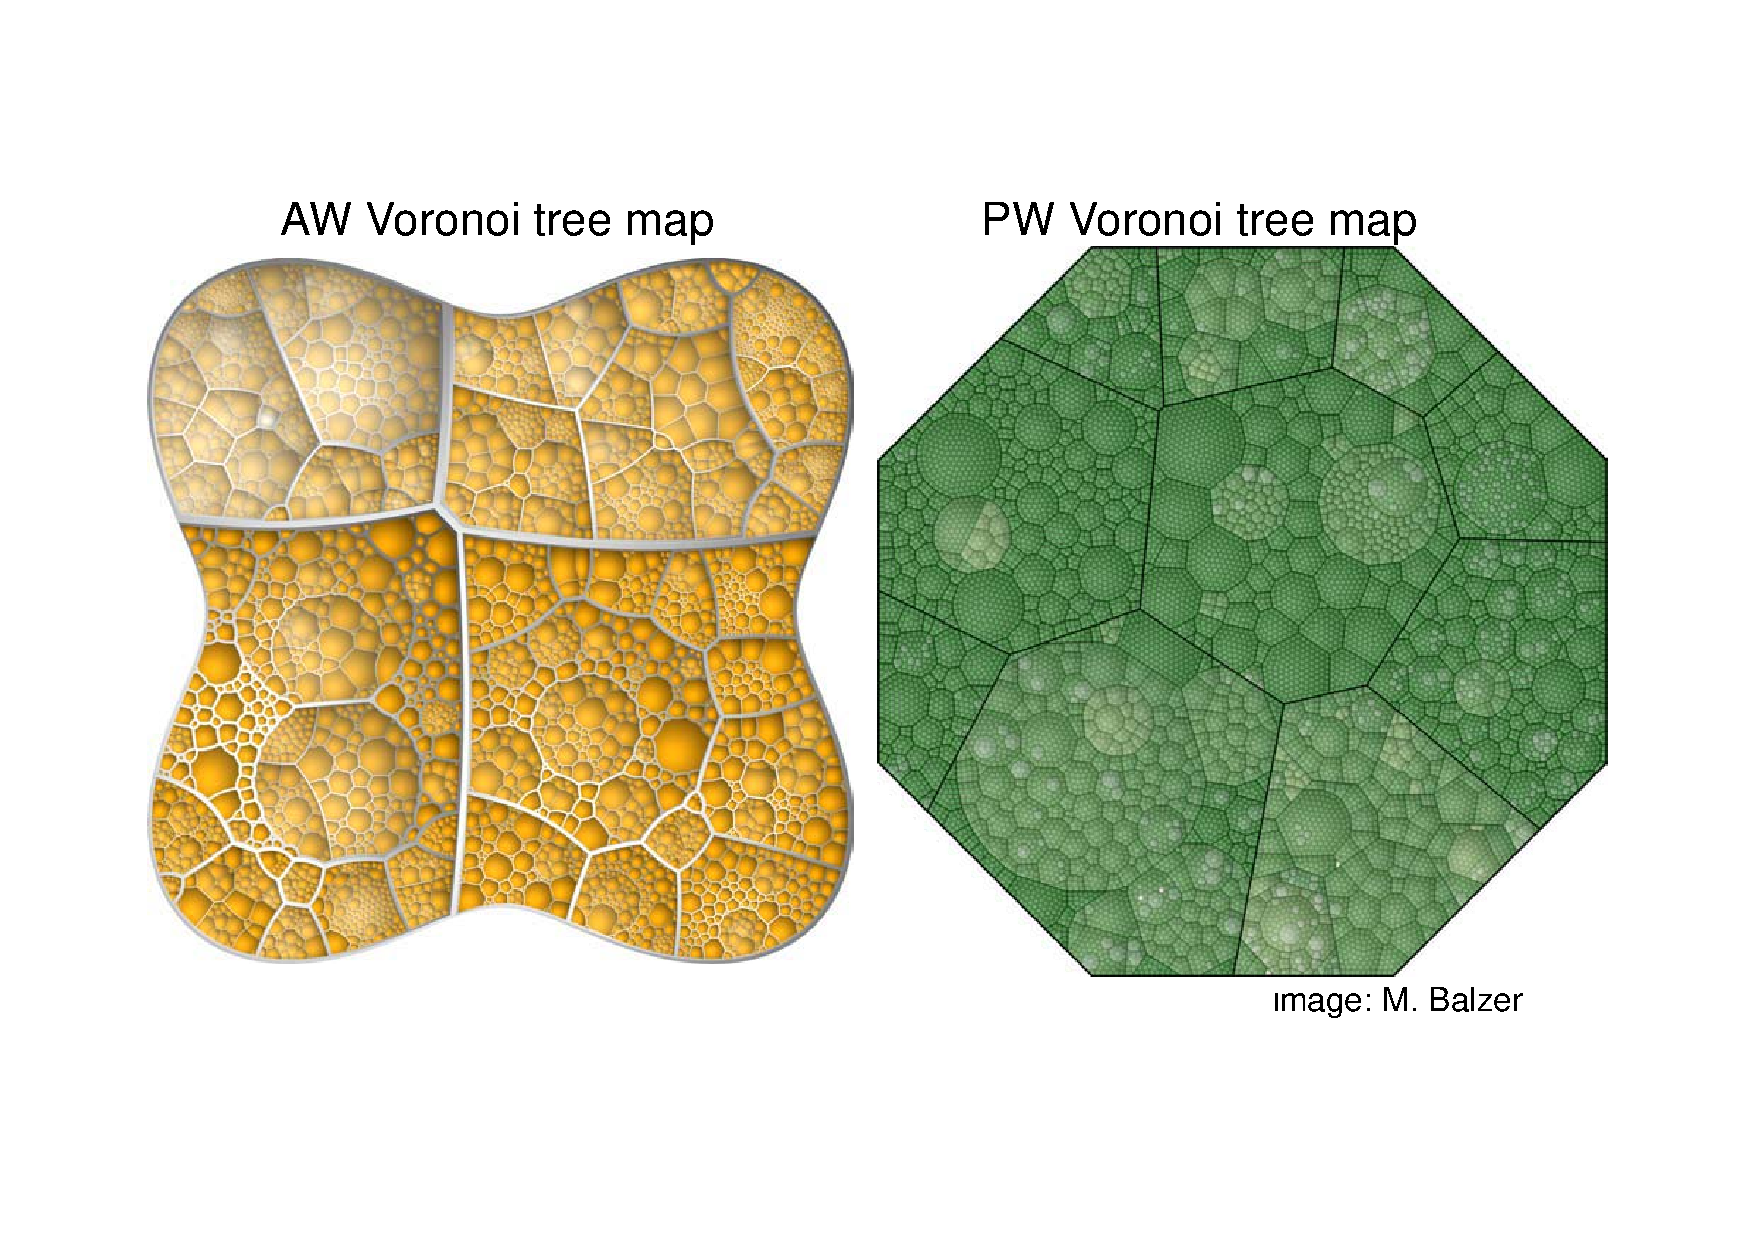
\includegraphics[width=0.7\textwidth]{img/12_voronoi_tree_map}
\end{figure}

\subsection{Clustering Techniques}
Motivation for \emph{clustering} in visualisation of graphs: Multiple levels-of-detail are obtained by identifying  "highly connected" subsets and representing the by glyphs.

Clustering techniques are often based on \emph{force models}. Assume an undirected graph $G=(V,E)$ with a set of nodes $V$ and a set of Edges $E$.

Notation:
\begin{description}
    \item $e_{ij}$ Edge connecting nodes $i$ and $j$.
    \item $p_i$ Position of node $i$
    \item $p_{ij} = \norm{p_i-p_j}$ 
\end{description}


The \emph{attractive force} is usually \emph{Hooke's spring law}
\begin{align*}
 f(x) = A\cdot(x-x_0),
\end{align*}
where $x_0$ is the zero energy length of the spring.

The \emph{repulsive force} generally follows an inverse square law inspired by \emph{electrostatic fields}:
\begin{align*}
    g(x) = {B\over x^2}.
\end{align*}
The total \emph{potential energy} is then:
\begin{align*}
    P = {A \over 2} \sum_{e_{ij} \in E} (p_{ij} - x_0)^2 - B\sum_{i\neq j} {1\over p_{ij}}.
\end{align*}

Difficult to visualise: \emph{Small world} graphs (Watts and Strogatz).

\paragraph{Small world graphs} are connect graphs having
\begin{itemize}
\item a small \emph{average path length} (between a pair of nodes) and
\item a high \emph{clustering index}
\end{itemize}
both compared to a random graph with the same number of nodes and edges.

The \emph{clustering index of a node} $v$ is the ratio between
\begin{itemize}
\item the number of \emph{existing} edges in the $1$-neighbourhood $N(v)$ of $v$.
\item the number of \emph{possible} edges, which is $k{k-1\over 2}$ if $k=|N(v)|$.
\end{itemize}

The \emph{clustering index of the graph} is the average of the clustering indices of its nodes.


Energy models suited for small-world problems:
$r$-PolyLog energy models (Noack):

\begin{description}
\item Potential Energy:
    \begin{align*}
        P = \sum_{e_{ij} \in E} (p_{ij} -x_0)^r - \sum_{j\neq i} \log (p_{ij}).
    \end{align*}
\item Attractive and repulsive forces are obtained by taking the derivative for $1$-Polylog:
\begin{align*}
 f(x) &= 1 \\
 g(x) &= {1\over x}
\end{align*}
\item Minimum energy configuration of $1$-PolyLog has the following property:
    
    Distance between two clusters $C_1$ and $C_2$ is inversely proportional to their \emph{coupling}:
    \begin{align*}
        {\left| 
            \left\{
                e_{ij}: i\in C_1, j\in C_2
            \right\}
         \right| \over
             |C_1|\ |C_2|
         }
    \end{align*}

\end{description}

\subsection{Distortion Techniques}

Various techniques:
\begin{itemize}
\item Perspective wall (Robertson)
\item Table lens (Rao and Card)
\end{itemize}

\subsubsection{Hyperbolic trees}
\emph{Hyperbolic trees} trees are based on the \emph{Poincaré Disk} model (projection) of the \emph{hyperbolic space $H_2$}.

In the Poincaré disk, the role of \emph{straight lines} is taken by:
\begin{itemize}
\item \emph{Circles} which intersect the bounding circle $x^2+y^2=1$ orthogonally
\item \emph{Diameters} of the bounding circle.
\end{itemize}

\paragraph{Properties} $\ $
\begin{itemize}
\item Triangles have the sum of angles $< 180º$.
\item It has the \emph{metric} 
    \begin{align*}
     ds = {\sqrt{dx^2+dy^2} \over 1-x^2-y^2}.
    \end{align*}
\item The bounding circle is at infinity
\item Circle perimeter grows exponentially with its radius.

    As a consequence trees can be drawn \emph{undistorted} in hyperbolic space:
    \begin{itemize}
        \item All edges having about the same length \emph{and}
        \item All nodes having the same angle available for their children.
    \end{itemize}
\end{itemize}

Rigid transformations of the Poincaré disk: \emph{Möbius transformations} of complex numbers:

\begin{align*}
 z'= T_{c\theta} (z) &= {\theta z + c\over \overline c \theta z + 1}, &
     |\theta| = 1,\ |c| < 1 
\end{align*}
These are:
\begin{description}
\item for $c=0$: \emph{rotations} around $0$.
\item for $\theta=1$: \emph{translations} (mapping $0$ to $c$ and $-c$ to $0$).
\item Combinations:
    \begin{align*}
        T_{c_2\theta_2}(T_{c_1\theta_1}(z)) = T_{c\theta} (z)
    \end{align*}
    with
    \begin{align*}
     c= {\theta_2 c_1 + c_2\over \theta_2 c_1 \overline c_2 + 1}, \qquad\quad \theta = {\theta_1\theta_2 + \theta_1\overline c_1 c_2\over \theta_2 c_1 \overline c_2 + 1}.
    \end{align*}

\end{description}

\paragraph{Technique} (Lamping et al) Change of focus, i.e. moving a different node towards the center, is achieved by performing a \emph{translation} in hyperbolic space. 

Example: Visualisation of a large organisational hierarchy in hyperbolic space with different foci.

\begin{figure}[H]
\centering
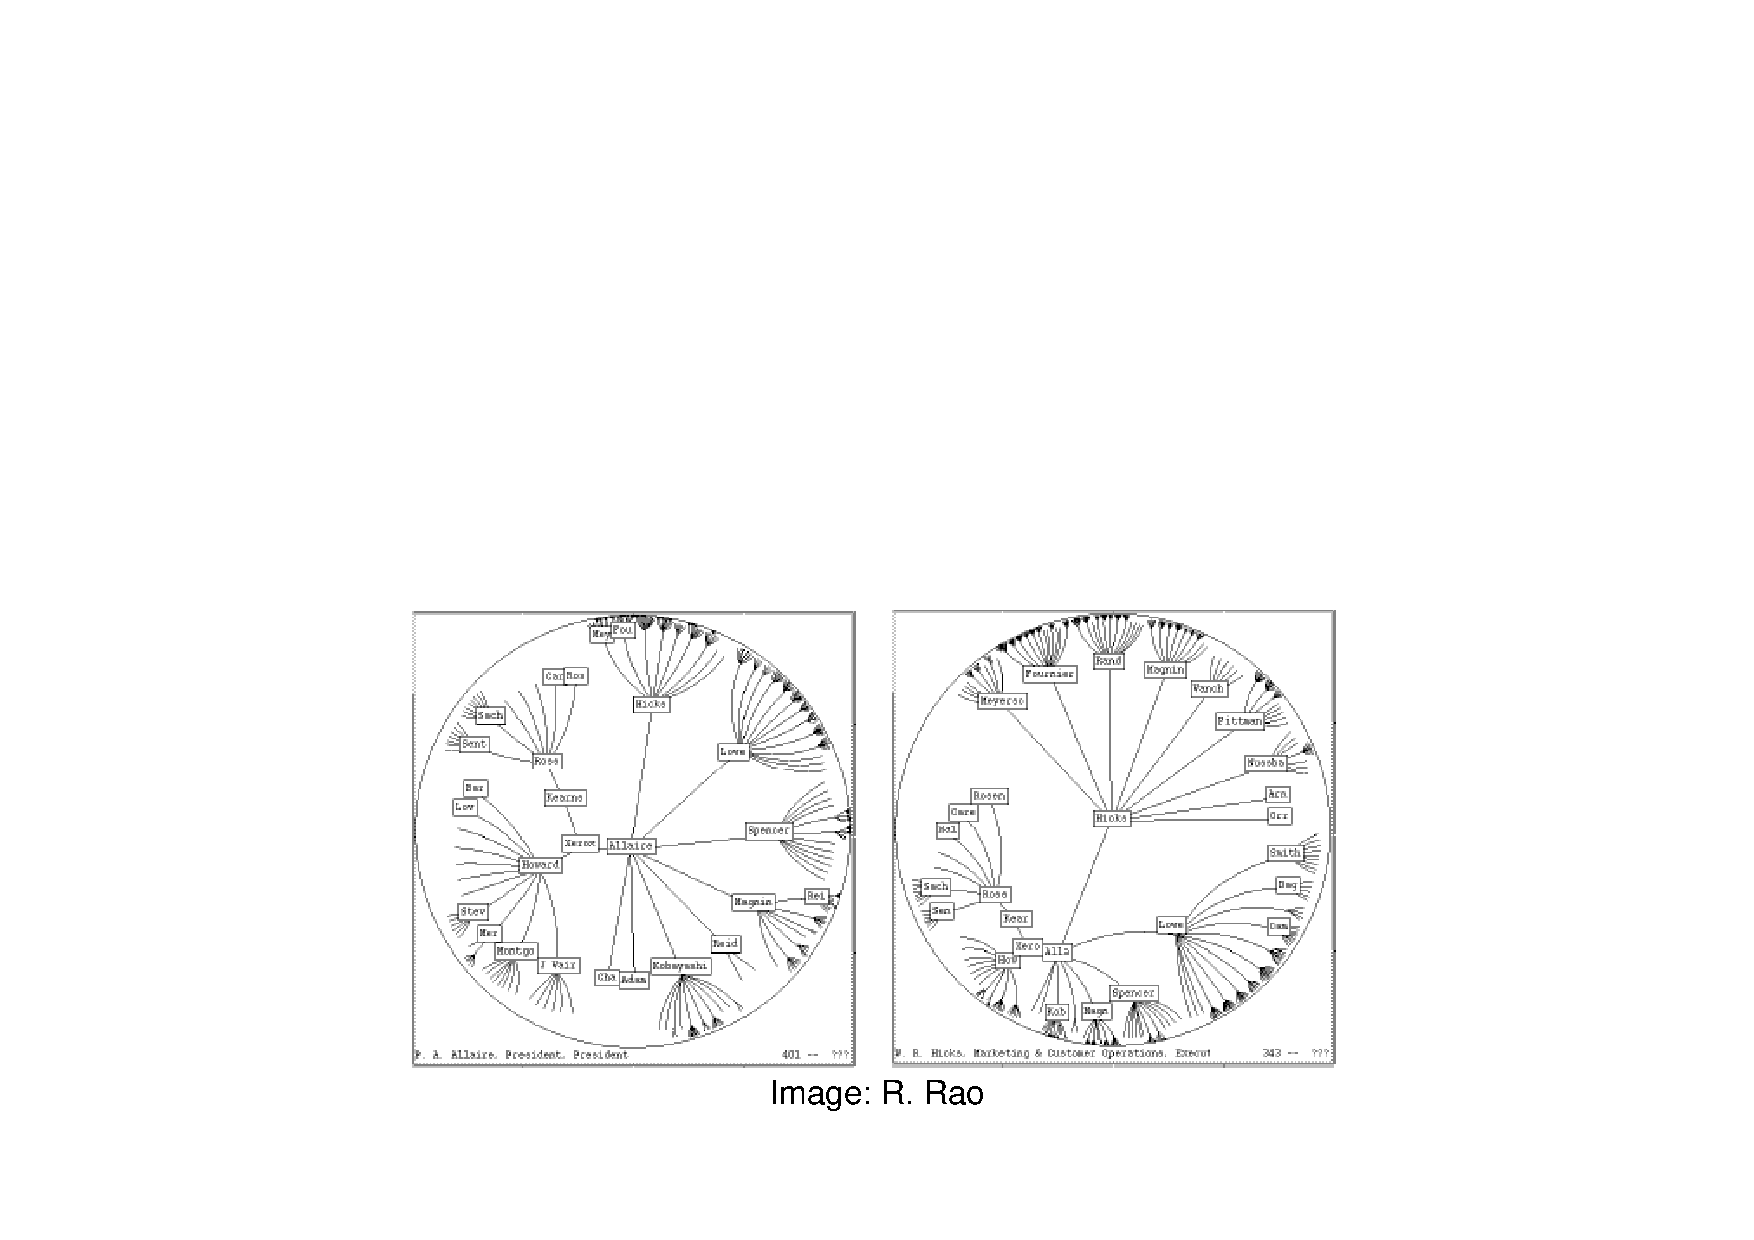
\includegraphics[width=0.7\textwidth]{img/12_hyperbolic_tree}
\end{figure}
